%!TEX root=seke.tex
% mainfile: ../seke.tex

\vspace*{-.075in}
\section{The IAdapter Testbed system}\label{sec:technique}
\vspace*{-.075in}


In this section, We devise a new testbed that has the ability to reproduce different types of web workloads.  The proposed solution extends a tool named IAdapter to create a testbed tool to validade load, performance and stress search based test approaches \cite{Gois2016}. This new testbed must accomplish three main goals. First, it must reproduce a workload by using an antipattern implementation. Second, it must be able to provide metrics with the aim of being used for research evaluation studies. Finally, it should be extensible, allowing the creation of new metaheuristic approaches.

The testbed tool proposed consists of four main modules.  Figure \ref{fig:testbedarch} presents the main architecture of the Testbed solution proposed. The emulator module provides workloads to the Test module. The Test module uses a class loader to find all classes that extends AbstractAlgorithm in the classpath and run all workloads with each metaheuristic found. The Test Scenario library provides the scenario representation used by the metaheuristics and store the testbed results in a database. The Operation services are responsible for finding neighbors of some workload provided as a parameter and perform crossover operations.

\begin{figure}[h]
\centering
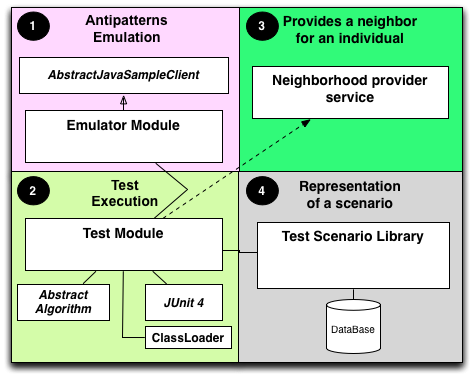
\includegraphics[width=0.5\textwidth]{./images/testbedarch.png}
\caption{Testbed main architecture.}
\label{fig:testbedarch}
\end{figure} 

\begin{figure}[h]
\centering
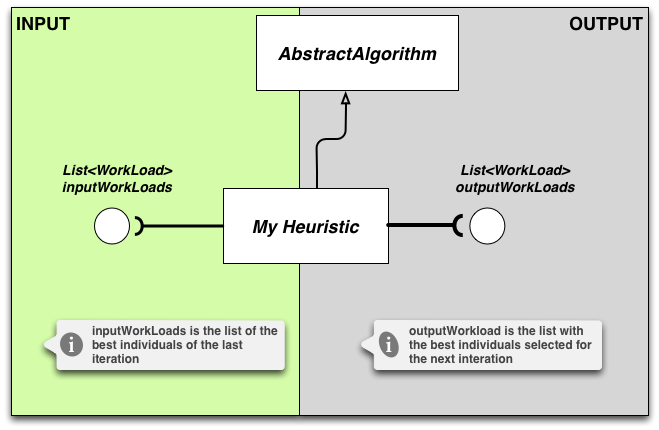
\includegraphics[width=0.5\textwidth]{./images/myheuristic.png}
\caption{Test Module class diagram.}
\label{fig:heuristicclassdiagram}
\end{figure} 



\subsection{Test Module}

The Test Module (Figure \ref{fig:testbedarch}  -\ding{202}) is responsible for for the loading of all classes that extend AbstractAlgorithm in the classpath and perform the tests under the application. Figure \ref{fig:heuristicclassdiagram} shows the  class diagram for custom and provided heuristics. All heuristic classes extends the class AbstractAlgorithm. The heuristics receives  as input a  list of workloads (Figure \ref{fig:heuristicclassdiagram}  -\ding{203}) and must return a list of output workloads (the individuals selected for the next generation)  (Figure \ref{fig:heuristicclassdiagram}  -\ding{204}). Each workload represent an individual in the search space. Figure. \ref{fig:step2} presents the Test Module life cycle. Given an initial population (Figure \ref{fig:step2}  -\ding{202}),  a metaheurist select a new set of workloads based on an objective function (Figure \ref{fig:step2}  -\ding{203}). The choosen metaheurist generate a new set of individuals based on crossover or neighborhood operators (Figure \ref{fig:step2}  -\ding{204}).  JMeterEngine run each workload (Figure \ref{fig:step2}  -\ding{206}) and the choosen metaheuristic obtain a fitness value for each workload based on some objective function  (Figure \ref{fig:step2}  -\ding{207}). Each Metaheuristic could define your own objective function. After all these steps the cycle begins until the maximum number of generations it is reached (Figure \ref{fig:step2}  -\ding{208}). 

\begin{figure}[h]
\begin{minipage}{.5\textwidth}
\centering
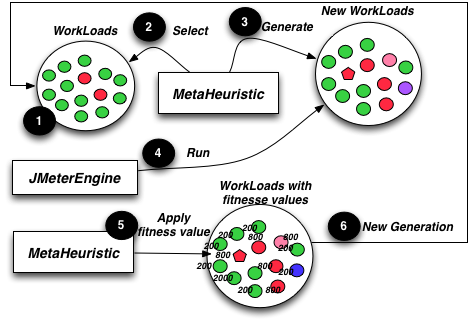
\includegraphics[width=1\textwidth]{./images/step2.png}
\caption{Test module life cycle.}
\label{fig:step2}
\end{minipage}
\end{figure} 



\subsection{Emulator Module}

The Emulator Module is responsible for implementing and providing successful scenarios and the most common performance antipatterns (Figure \ref{fig:testbedarch}  -\ding{203}). All classes must extend the AbstractJavaSamplerClient class or use JUnit 4. The AbstractJavaSamplerClient class allows the creation of a JMeter Java Request. Figure \ref{fig:emulator} presents the main features of the emulator module. The module implements 2 happy scenarios (Figure \ref{fig:emulator}  -\ding{203}) and  4 antipatterns test scenarios (Figure \ref{fig:emulator}  -\ding{202}), in its first version. The Mock Layer provides emulated databases and components for the test scenarios. The Mock Layer use the Mockito and PowerMocks frameworks (Figure \ref{fig:emulator}  -\ding{204}). 

\begin{figure}[h]
\centering
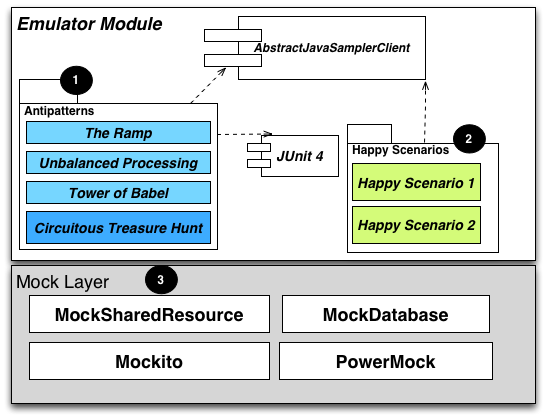
\includegraphics[width=0.5\textwidth]{./images/emulator.png}
\caption{Emulator module}
\label{fig:emulator}
\end{figure}  

\subsection{Test Scenario Library}

This modules provides a common representation for all workloads (Figure \ref{fig:testbedarch}  -\ding{205}). Each workload is composed by a linear vector with 21 positions (Figure \ref{fig:solution}  -\ding{202}). The first position represents an metadata with the name of an individual. The next positions represent 10 scenarios and their numbers of users (Figure \ref{fig:solution}  -\ding{203}). Each scenario is an atomic operation: the scenario must log into the application, run the task goal, and undo any changes performed, returning the application to its original state. 

\subsection{Operation services}

The services are responsible for performing some operations performed by metaheuristics. Figure. \ref{fig:solution} presents the solution representation and an example using the crossover operation. In the example, solution 1 (Figure \ref{fig:solution}  -\ding{204}) has the Login scenario with 2 users, the Search scenario with 4 users, Include scenario with 1 user and the Delete scenario with 2 users.  After the crossover operation with solution 2 (Figure \ref{fig:solution}  -\ding{205}), We obtain a solution with the Login scenario with 2 users, the Search scenario with 4 users, the Update scenario with 3 users and the Include scenario with 5 users (Figure \ref{fig:solution}  -\ding{206}). Figure. \ref{fig:solution} -\ding{207} shows the strategy used by the proposed solution to  obtain the neighbors for the Tabu search and simulated annealing algorithms. The neighbors are obtained by the modification of a single position (scenario or number of users) in the vector.


\begin{figure}[h]
\centering
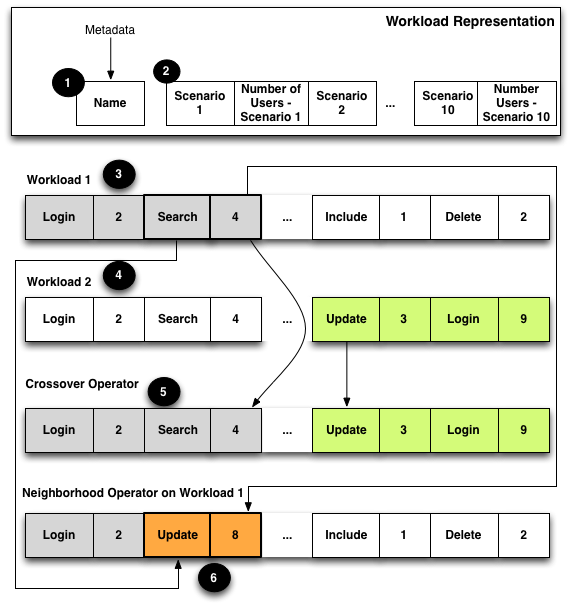
\includegraphics[width=0.5\textwidth]{./images/genomere.png}
\caption{Solution representation, crossover  and neighborhood operators}
\label{fig:solution}
\end{figure}



\section{Experiments}

In this section, We present the results of experiments which we carried out to verify the antipatterns  implementation and the metaheuristics used by the testbed tool. We conducted two experiments in order to verify the effectiveness of the testbed tool. Each experiment use two different antipatterns and the happy scenarios. The experiments ran for 17 generations. The experiments used an initial population of 4 individuals by metaheuristic. The genetic algorithm used the top 10 individuals from each generation in the crossover operation. The Tabu list was configured with the size of 10 individuals and expired every 2 generations.  The mutation operation was applied to 10\% of the population on each generation. The experiments uses tabu search, genetic algorithms and the hybrid metaheuristic approach proposed by Gois et al. \cite{Gois2016}. The objective function applied is intended to maximize the number of users and minimize the response time of the scenarios being tested.  In this experiments, better fitness values means to find scenarios with more users and lower values of a response time. A penalty is applied when the response time is greater than the  maximum response time expected. 

\subsection{Experiment Research Questions}

The following research question is addressed:
\begin{itemize*}
\item Does the IAdapter testbed correctly emulates an antipattern?
\item Does the IAdapter testbed be able to provide metrics with the aim of being used for stress search-based evaluation studies? 
\item Is the IAdapter testbed extensible, allowing the use of several metaheuristic approaches?
\end{itemize*}

\subsection{Variables}

The independent variables are the test scenarios (antipatterns and happy scenarios). The dependent variable are: the number of antipatterns found in best workloads and the metaheuristic with the best fitness value.

\subsection{Hypotheses}

\begin{itemize}
\item With regard to antipatterns implementation or emulation:
\begin{itemize*}
\item $H_{0}$ (A null hypothesis) :the best workloads found in the experiments contain antipatterns
\item $H_{1}$  : the best workloads found in the experiments do not contain antipatterns.
\end{itemize*}
\end{itemize}

\begin{itemize}
\item With regard to metrics provided by the IAdapter:
\begin{itemize*}
\item $H_{0}$ (A null hypothesis) : The IAdapter testbed does not be able to provide metrics with the aim of being used for stress search-based evaluation studies.
\item $H_{1}$  : The IAdapter testbed is able to provide metrics with the aim of being used for stress search-based evaluation studies.
\end{itemize*}
\end{itemize}

\begin{itemize}
\item With regard to the IAdapter testbed customization:
\begin{itemize*}
\item $H_{0}$ (A null hypothesis) :the IAdapter testbed is not extensible, disallowing the use of several metaheuristic approaches.
\item $H_{1}$  : the IAdapter testbed is extensible, allowing the use of several metaheuristic approaches.
\end{itemize*}
\end{itemize}

\subsection{The Ramp and Circuitous Treasure Hunt experiment}

The experiment was carried out for 8 continuous hours.  All tests in the experiment were conducted without the need of a tester, automating the process of executing and designing performance test scenarios.In this experiment, Scenarios were generated with the Ramp and Circuitous Treasure antipattern as well as scenarios with Happy Scenario 1, Happy Scenario 2 and mixed scenarios. Figure \ref{fig:boxplot1} present the fitness value obtained by each metaheuristic.

\begin{figure}[h]
\begin{minipage}{.5\textwidth}
\centering
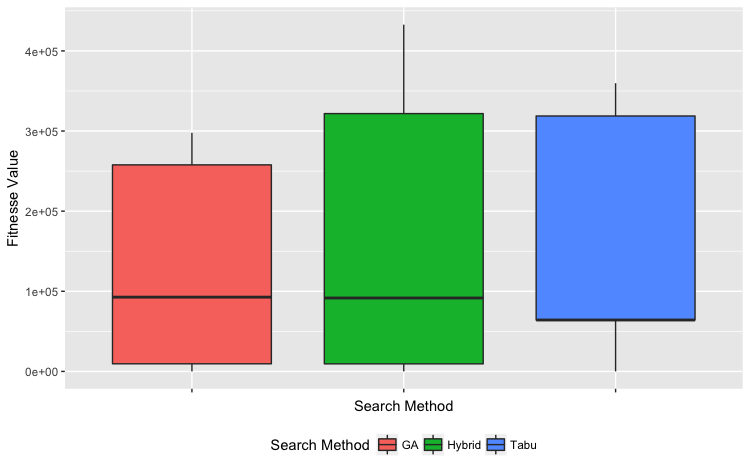
\includegraphics[width=0.8\textwidth]{./images/experiment1-4.png}
\caption{Average, median, maximum and minimal fitness value by Search Method}
\label{fig:boxplot1}
\end{minipage}
\end{figure}

Table \ref{tab:bestindividuals} shows 4 best individuals found in the experiment. None of the best individuals has one of the antipatterns used in the experiment, excluding the scenarios with antipatterns. 

% Please add the following required packages to your document preamble:
% \usepackage[table,xcdraw]{xcolor}
% If you use beamer only pass "xcolor=table" option, i.e. \documentclass[xcolor=table]{beamer}
\begin{table}[h]
\centering
\caption{Best individuals found in the first experiment}
\label{tab:bestindividuals}
\begin{tabular}{lllll}
\rowcolor[HTML]{C0C0C0} 
\textbf{Metaheur.} & \textbf{Gen.} & \textbf{Users} & \textbf{Fit} & \textbf{Scenarios}  \\
Hybrid & 17 & 145 & 432760 & Happy 1 \& 2  \\
Hybrid & 17 & 145 & 432740 & Happy 1 \& 2   \\
Hybrid & 17 & 146 & 431760 & Happy 1 \& 2  \\
Hybrid & 16 & 143 & 426740 & Happy 1 \& 2  
\end{tabular}
\end{table}


\vspace*{-.075in}
\subsection{The Tower Babel  and Unbalanced Processing experiment}
\vspace*{-.075in}

The experiment was carried out for 6 continuous hours. In this experiment, Scenarios were generated with Tower Babel and Unbalanced Processing antipattern as well as scenarios with Happy Scenario 1, Happy Scenario 2 and mixed scenarios.

\begin{figure}[h]
\begin{minipage}{.5\textwidth}
\centering
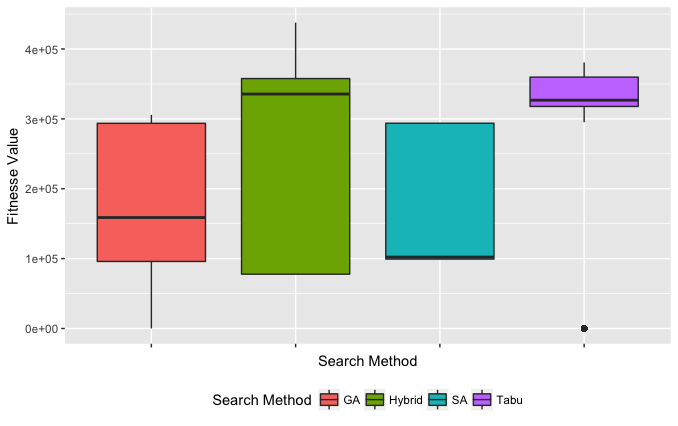
\includegraphics[width=0.8\textwidth]{./images/experiment2-2.png}
\caption{Finesse value by generation in all tests}
\label{fig:boxplot2}
\end{minipage}

\end{figure}



Table \ref{tab:bestindividuals2} shows the 4 best workloads found in the second experiment. Despite the fact of doing 300 conversions of the JSON format to XML. The antipattern implementation does not return a higher response time than happy paths. While happy paths returns from 10 to 15 seconds from a single user, Tower Babel antipattern has a response time of 10 to 29 seconds. None of the best individuals found implements the Unbalanced Processing antipattern.


% Please add the following required packages to your document preamble:
% \usepackage[table,xcdraw]{xcolor}
% If you use beamer only pass "xcolor=table" option, i.e. \documentclass[xcolor=table]{beamer}
\begin{table}[h]
\centering
\caption{Best individuals found in the second experiment}
\label{tab:bestindividuals2}
\begin{tabular}{lllll}
\rowcolor[HTML]{FFCCC9} 
\textbf{Metaheur.} & \textbf{Gen.} & \textbf{Users} & \textbf{Fit} & \textbf{Scenarios}  \\ 
\multicolumn{1}{l}{Hybrid} & \multicolumn{1}{l}{17} & \multicolumn{1}{l}{148} & \multicolumn{1}{l}{437780} & \multicolumn{1}{l}{Happy 1,2 \& Tower}  \\ 
\multicolumn{1}{l}{Hybrid} & \multicolumn{1}{l}{17} & \multicolumn{1}{l}{145} & \multicolumn{1}{l}{432740} & \multicolumn{1}{l}{Happy 1,2 \& Tower}  \\ 
\multicolumn{1}{l}{Hybrid} & \multicolumn{1}{l}{16} & \multicolumn{1}{l}{146} & \multicolumn{1}{l}{431800} & \multicolumn{1}{l}{Happy 1,2 \& Tower} \\ 
\multicolumn{1}{l}{Hybrid} & \multicolumn{1}{l}{17} & \multicolumn{1}{l}{145} & \multicolumn{1}{l}{428780} & \multicolumn{1}{l}{Happy 1,2 \& Tower}  \\ 
\end{tabular}
\end{table}

In the second experiment, the metaheuristics converged to scenarios with a happy path and Tower Babel antipattern, excluding the scenarios with Unbalanced Processing antipattern. The hybrid metaheuristic returned individuals with higher fitness scores. The SA algorithm obtained the worst fitness values. 

\subsection{Threats to validity}
\begin{itemize*}
\item Construct Validity: 
In this work, we just evaluate the use of four antipatterns. However, several antipatterns could be applied.  The testbed's common representation and the strategies used for crossover and neighborhood operators need of a better design, using an abstraction pattern to contemplate a major number of possible solutions.
\item Conclusion Validity: 
The Tower Babel antipattern was not excluded by the metaheuristics used in the experiment, requiring new studies with new approaches and experiments.
\end{itemize*}




\vspace*{-.075in}
\section{Conclusion}
\vspace*{-.075in}

IAdapter Testbed is an open-source facility that provides software tools for search based test research. The testbed tool emulates test scenarios in a controled environment using mock objects and implementing performance antipatterns.  Two experiments were conducted to validate the proposed approach. The experiments use genetic, algorithms, tabu search, simulated annealing and a new hybrid approach proposed by Gois et al. \cite{Gois2016}. In the first experiment, none of the best workloads has one of the antipattern scenarios. In the second experiment,  the metaheuristics converged to scenarios with an happy path and Tower Babel antipattern, excluding the scenarios with Unbalanced Processing antipattern. In both experiments the hybrid metaheuristic returned individuals with higher fitness scores. Future works include the use of new antipatterns and more experiments with the use of the Tower Babel antipattern.